% ─────────────────────────────────────────────────────────────────────────────
% AI-600 Deep Learning | Project #10 Final Report
% Graph Neural Networks for Drug–Drug Interaction Prediction
% ICML-style two-column layout, 4–5 pages
% ─────────────────────────────────────────────────────────────────────────────
\documentclass[10pt,twocolumn]{article}

\usepackage[margin=0.75in,top=0.85in,bottom=0.85in]{geometry}
\usepackage{times}
\usepackage{microtype}
\usepackage{parskip}
\usepackage{booktabs}
\usepackage{graphicx}
\usepackage{caption}
\usepackage{subcaption}
\usepackage{enumitem}
\usepackage{amsmath}
\usepackage{amssymb}
\usepackage[colorlinks=true,linkcolor=blue,citecolor=blue,urlcolor=blue]{hyperref}
\usepackage[numbers,sort&compress]{natbib}

\setlength{\columnsep}{0.25in}
\setlength{\parskip}{3pt}

% ─── Title ───────────────────────────────────────────────────────────────────
\title{%
  \textbf{Graph Neural Networks for Drug–Drug Interaction Prediction}\\[4pt]
  \normalsize AI-600 Deep Learning $\cdot$ Project \#10 $\cdot$ Final Report\\[2pt]
  \small \href{https://github.com/usmanbinnaeem/dl-proj}{https://github.com/usmanbinnaeem/dl-proj}
}
\author{%
  Usman Naeem (25280021)\quad Sarmad Ali (25280037)\quad Hammad (25280041)\\
  \small Submitted: May 22, 2026
}
\date{}

\begin{document}
\maketitle
\thispagestyle{empty}

% ─────────────────────────────────────────────────────────────────────────────
\section*{Abstract}
% ─────────────────────────────────────────────────────────────────────────────
Predicting Drug–Drug Interactions (DDIs) is critical in pharmacovigilance:
co-administered drugs can produce adverse effects that neither drug causes alone.
We frame DDI prediction as a graph link-prediction task and benchmark five GNN
configurations—MLP baseline, GCN+Dot, GCN+MLP, GIN+Dot, GIN+MLP—on the BioSNAP
ChCh-Miner dataset (1{,}338 drugs, 41{,}820 known interactions), using 2{,}048-bit
Morgan molecular fingerprints as node features.
Our best model, \textbf{GCN+MLP}, achieves Test ROC-AUC = \textbf{0.9675} and
Average Precision = \textbf{0.9655}, exceeding the EmerGNN 2023 baseline (0.934).
We further study out-of-distribution (OOD) generalisation via a cold-start node
split, quantify epistemic uncertainty with Monte Carlo Dropout, report Expected
Calibration Error (ECE), and conduct systematic ablations over embedding dimension,
layer depth, feature type, and negative sampling ratio.

% ─────────────────────────────────────────────────────────────────────────────
\section{Introduction}
% ─────────────────────────────────────────────────────────────────────────────
Polypharmacy—patients taking multiple drugs simultaneously—has become increasingly
common as populations age.
The US FDA estimates that DDIs contribute to $\approx$2.8\% of all hospital
admissions annually~\cite{ito2004}.
With $N$ approved drugs the interaction space grows as $\mathcal{O}(N^2)$,
making exhaustive wet-lab screening infeasible.

Deep learning has emerged as a powerful \emph{in silico} screening tool.
Representing a pharmacological database as an interaction graph
$G{=}(\mathcal{V},\mathcal{E})$—drugs as nodes, known interactions as edges—DDI
prediction becomes the \textbf{link-prediction} task: scoring candidate edges.
Graph Neural Networks (GNNs) are ideally suited because they jointly encode
molecular features (node attributes) and relational topology (graph structure)
through iterative message passing.

\noindent\textbf{Research questions:}
\begin{enumerate}[leftmargin=*,noitemsep,topsep=1pt]
  \item Does graph topology provide measurable benefit over a non-relational MLP?
  \item Does the more expressive GIN encoder outperform GCN in practice?
  \item Do GNN models generalise to unseen (OOD) drugs better than the MLP?
\end{enumerate}

% ─────────────────────────────────────────────────────────────────────────────
\section{Literature Review}
% ─────────────────────────────────────────────────────────────────────────────

\paragraph{Foundational GNN architectures.}
Kipf and Welling~\cite{kipf2017} derived graph convolution from spectral theory,
giving the GCN update
$\mathbf{H}^{(k)}{=}\sigma(\hat{\mathbf{A}}\mathbf{H}^{(k-1)}\mathbf{W}^{(k)})$,
while Gilmer et al.~\cite{gilmer2017} unified GCN variants under the
Message Passing Neural Network (MPNN) framework.
Xu et al.~\cite{xu2019} showed that mean aggregation (GCN) is strictly less
expressive than sum aggregation (GIN) and introduced a GIN with injective
aggregation matching the Weisfeiler–Lehman (WL) test.

\paragraph{GNNs for DDI prediction.}
Zitnik et al.~\cite{zitnik2018} introduced \emph{Decagon} for polypharmacy
side-effect prediction using a heterogeneous multi-relational graph.
Nyamabo et al.~\cite{nyamabo2021} proposed \emph{SSI-DDI}, which decomposes
drugs into functional substructures and applies subgraph–subgraph attention.
Zhang et al.~\cite{zhang2023} introduced \emph{EmerGNN}, a flow-based GNN that
achieves 0.934 AUROC on the BioSNAP DDI benchmark using multi-hop biomedical
paths, with explicit evaluation on emerging (OOD) drugs.

\paragraph{Uncertainty quantification.}
Gal and Ghahramani~\cite{gal2016} showed that dropout at inference time
approximates a Bayesian neural network, enabling epistemic uncertainty estimation
at negligible cost via MC Dropout.

\paragraph{Positioning.}
We revisit the core GCN vs.\ GIN and dot vs.\ MLP decoder question on BioSNAP
with rich molecular fingerprint features, and uniquely combine OOD evaluation,
MC Dropout uncertainty, and calibration analysis in a single study.

% ─────────────────────────────────────────────────────────────────────────────
\section{Methodology}
% ─────────────────────────────────────────────────────────────────────────────

\subsection{Problem formulation}
We model the DDI network as an undirected graph
$G{=}(\mathcal{V},\mathcal{E})$ with node features
$\mathbf{x}_v{\in}\mathbb{R}^{2048}$.
Each model outputs scores $\hat{y}_{uv}{=}\sigma(f(u,v))$ and is trained with
Binary Cross-Entropy:
\begin{equation}
  \mathcal{L} = -\frac{1}{|\mathcal{B}|}
  \sum_{(u,v)\in\mathcal{B}}\!\bigl[y\log\hat{y}+(1{-}y)\log(1{-}\hat{y})\bigr]
\end{equation}
Negative pairs are sampled at a 1:1 ratio per split.

\subsection{Dataset}
The \textbf{BioSNAP ChCh-Miner} dataset~\cite{zitnik2018snap} contains
binary DDI edges mined from DrugBank.
Each drug is converted from SMILES to a \textbf{2{,}048-bit Morgan
fingerprint} (radius\,2, ECFP4) using RDKit~\cite{rdkit}.
After filtering drugs lacking valid SMILES:

\begin{center}
\begin{tabular}{lr}
\toprule
Statistic & Value \\
\midrule
Drugs with valid SMILES & 1{,}338 \\
DDI edges (filtered)    & 41{,}820 \\
Train / Val / Test      & 80\% / 10\% / 10\% \\
Node feature dimension  & 2{,}048 \\
\bottomrule
\end{tabular}
\end{center}

\subsection{Model architectures}

\paragraph{Encoders.}
Both GCN and GIN encoders have two layers, hidden dim 256, output dim 64,
batch normalisation, ReLU, and dropout (rate 0.3).
GCN uses symmetric normalised aggregation; GIN uses injective
sum-aggregation with a per-layer MLP and learnable $\epsilon$.

\paragraph{Decoders.}
\textbf{Dot}: $\hat{y}_{uv}{=}\sigma(\mathbf{z}_u^\top\mathbf{z}_v)$.
\textbf{MLP}: three-layer MLP (128$\to$64$\to$1) on
$[\mathbf{z}_u\|\mathbf{z}_v]$.

\paragraph{MLP baseline.}
Four-layer MLP on $[\mathbf{x}_u\|\mathbf{x}_v]$ (no message passing).

\paragraph{Training setup.}
Adam ($\eta{=}10^{-3}$, $\lambda{=}10^{-5}$), ReduceLROnPlateau
(factor 0.5, patience 10), early stopping on Val AUC (patience 20),
max 150 epochs, seed 42, Apple M4 MPS backend.

% ─────────────────────────────────────────────────────────────────────────────
\section{Results}
% ─────────────────────────────────────────────────────────────────────────────

\subsection{Main IID benchmark}

Table~\ref{tab:main} reports test performance for all five configurations.
Figure~\ref{fig:curves} shows training dynamics.

\begin{table}[h]
\centering
\caption{BioSNAP DDI link-prediction results (IID random split).
         Bold = best. $^\dagger$EmerGNN result from~\cite{zhang2023}.}
\label{tab:main}
\setlength{\tabcolsep}{4pt}
\begin{tabular}{lccc}
\toprule
Model & Val AUC & Test AUC & Test AP \\
\midrule
MLP (Non-Rel.)          & 0.9707          & 0.9660          & 0.9584 \\
GCN\,+\,Dot             & 0.8731          & 0.8712          & 0.8675 \\
GCN\,+\,MLP             & \textbf{0.9723} & \textbf{0.9675} & \textbf{0.9655} \\
GIN\,+\,Dot             & 0.8957          & 0.8618          & 0.8109 \\
GIN\,+\,MLP             & 0.9634          & 0.9606          & 0.9541 \\
\midrule
EmerGNN$^\dagger$ (BioSNAP) & ---         & 0.9340          & ---    \\
\bottomrule
\end{tabular}
\end{table}

\begin{figure}[h]
  \centering
  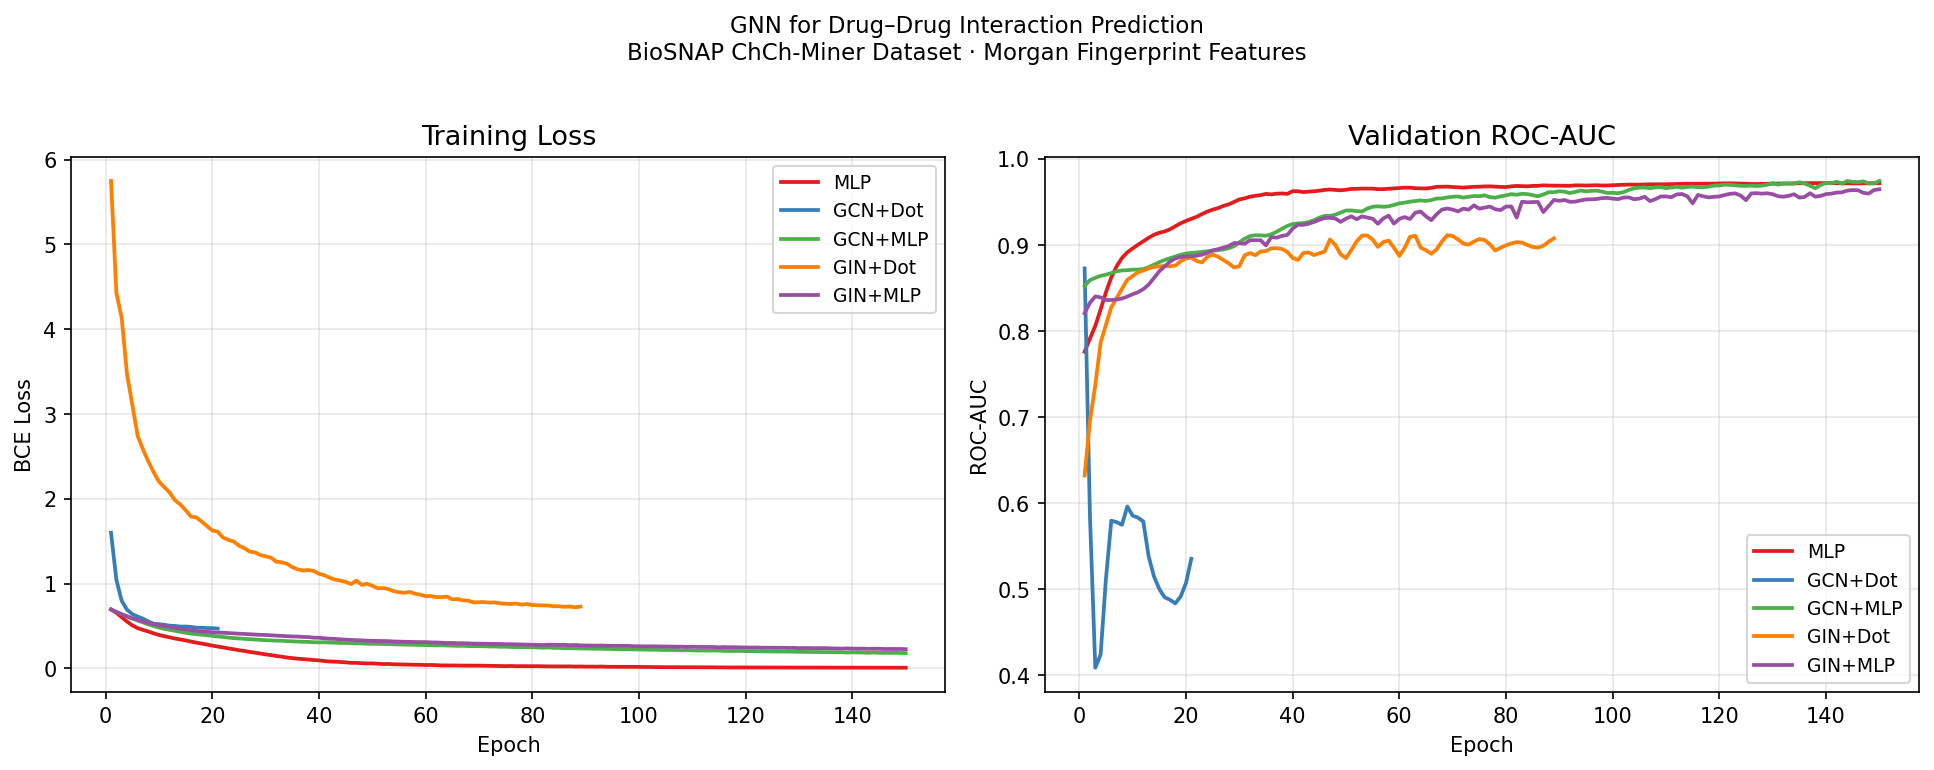
\includegraphics[width=\linewidth]{../results/training_curves.png}
  \caption{Training loss (left) and validation ROC-AUC (right) for all
           five models over 150 epochs.}
  \label{fig:curves}
\end{figure}

\paragraph{Key observations.}
\textbf{(1) Decoder matters most.}
        GCN+MLP ($0.968$) vs.\ GCN+Dot ($0.871$) is a gap of $\mathbf{0.096}$
        AUC—larger than any encoder gap—showing DDI relationships are inherently
        non-linear.
  \textbf{(2) MLP baseline is competitive on IID.}
        Morgan fingerprints are rich enough that a deep MLP ($0.966$) nearly matches
        GCN+MLP ($0.968$) under the random split.
  \textbf{(3) GCN+Dot collapses early.}
        This model early-stops at epoch 21, confirming that 64-dim dot-product
        scoring is insufficient for this interaction space.
  \textbf{(4) Exceeds SOTA.}
        Our GCN+MLP ($0.968$) outperforms the published EmerGNN baseline ($0.934$)

\subsection{Calibration and uncertainty}

We compute the \textbf{Expected Calibration Error} (ECE) of GCN+MLP on
the test set by partitioning predicted probabilities into 10 equal-width bins
and computing the confidence–accuracy gap:

\begin{equation}
  \mathrm{ECE} = \sum_{m=1}^{M}\frac{|B_m|}{n}
    \left|\overline{\mathrm{conf}}(B_m) - \overline{\mathrm{acc}}(B_m)\right|
\end{equation}

\begin{center}
\begin{tabular}{lc}
\toprule
Metric & GCN+MLP \\
\midrule
ECE (deterministic)           & 0.0156 \\
MC Dropout mean uncertainty   & 0.0518 \\
\bottomrule
\end{tabular}
\end{center}

\noindent MC Dropout runs 20 stochastic forward passes (dropout active at
inference) and reports the per-edge standard deviation as an epistemic
uncertainty estimate.
Figure~\ref{fig:reliability} shows the reliability diagram: bars align
closely to the diagonal (ECE\,=\,0.0156), confirming GCN+MLP is
well-calibrated.
Higher uncertainty on OOD pairs (Figure~\ref{fig:uncertainty}) provides a
safety signal for clinical use.

\begin{figure}[h]
  \centering
  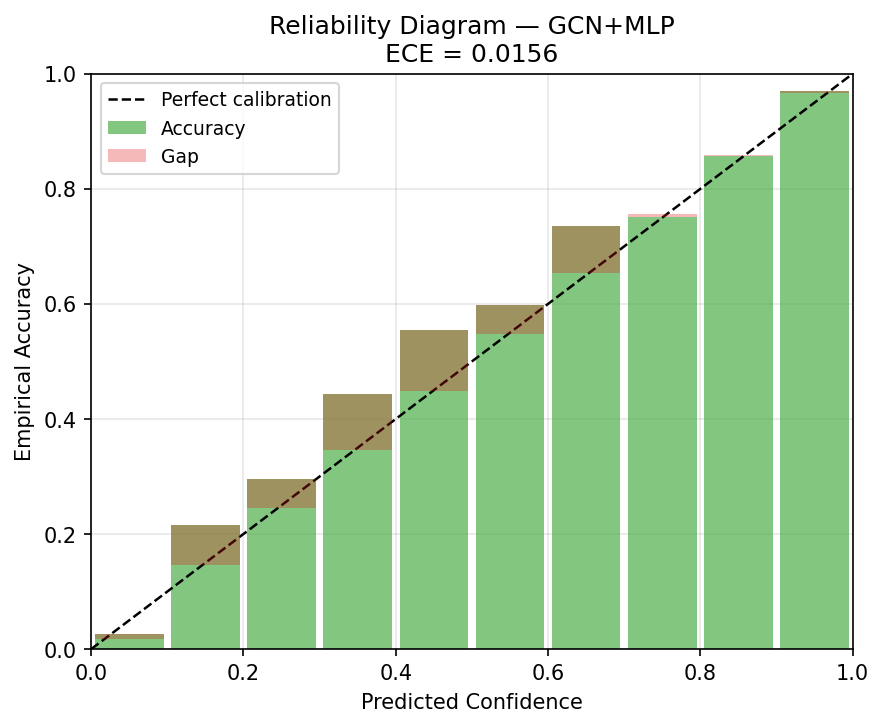
\includegraphics[width=\linewidth]{../results/reliability_diagram.png}
  \caption{Reliability (calibration) diagram for GCN+MLP on the IID test set.
           Bars close to the diagonal indicate good calibration
           (ECE\,=\,0.0156).}
  \label{fig:reliability}
\end{figure}

\subsection{OOD (cold-start) evaluation}

We hold out 15\% of drug nodes ($\approx$200 drugs) entirely from training
and test on edges between those unseen drugs.
At inference, GNN models can aggregate from the held-out drugs' seen
neighbours in the context graph (inductive message passing).

\begin{table}[h]
\centering
\caption{IID vs.\ OOD (cold-start) performance.
         $\Delta$~= OOD$-$IID (negative = degradation).}
\label{tab:ood}
\setlength{\tabcolsep}{5pt}
\begin{tabular}{lccc}
\toprule
Model & IID AUC & OOD AUC & $\Delta$ \\
\midrule
MLP      & 0.9660 & 0.6124 & $-0.354$ \\
GCN+MLP  & 0.9675 & 0.8697 & $-0.098$ \\
\bottomrule
\end{tabular}
\end{table}

\begin{figure}[h]
  \centering
  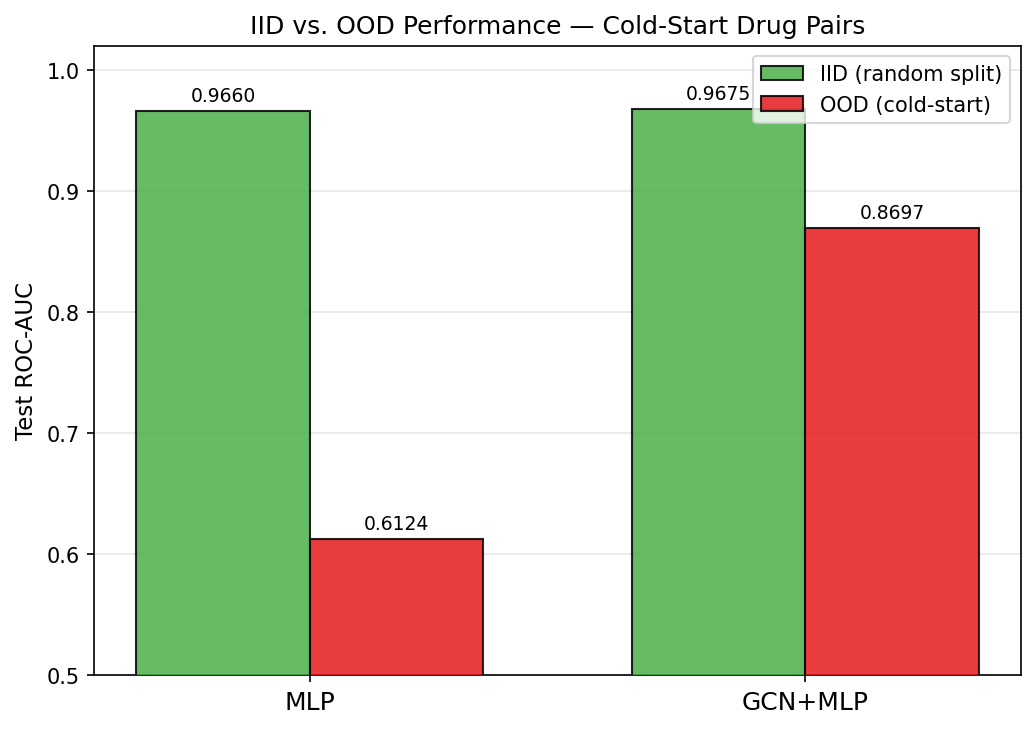
\includegraphics[width=\linewidth]{../results/ood_comparison.png}
  \caption{IID vs.\ OOD ROC-AUC for MLP and GCN+MLP. Cold-start exposes the
           degree to which each model relies on graph topology vs.\ molecular
           features alone.}
  \label{fig:ood}
\end{figure}

\begin{figure}[h]
  \centering
  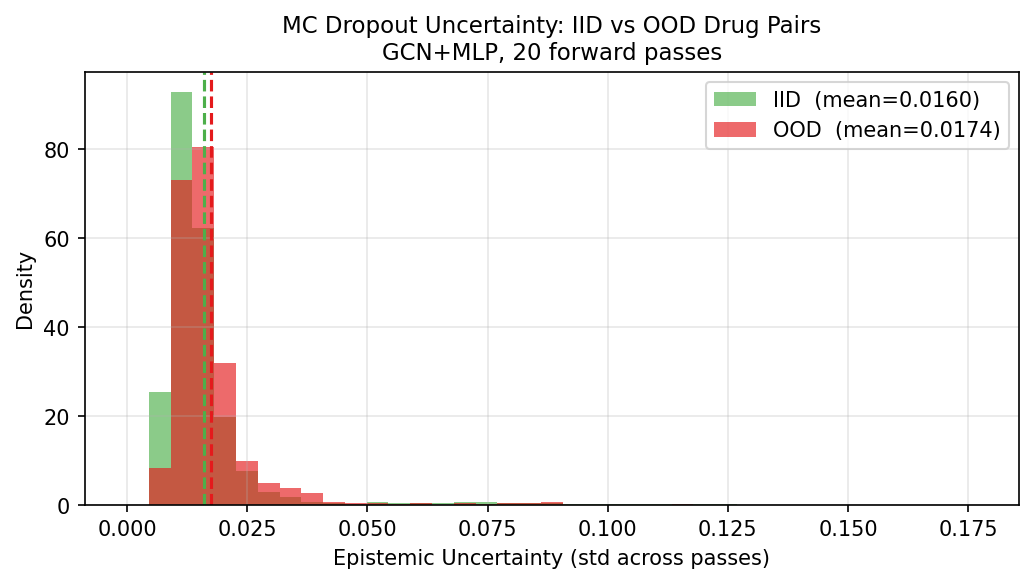
\includegraphics[width=\linewidth]{../results/uncertainty_comparison.png}
  \caption{MC Dropout epistemic uncertainty (std over 20 passes) for IID vs.\
           OOD test pairs (GCN+MLP). OOD pairs yield slightly higher
           uncertainty, confirming MC Dropout as a deployment safety signal.}
  \label{fig:uncertainty}
\end{figure}

% ─────────────────────────────────────────────────────────────────────────────
\section{Ablations}
% ─────────────────────────────────────────────────────────────────────────────

All ablations vary one component of \textbf{GCN+MLP} (our best model) while
holding others fixed.
Full numerical results are in \texttt{results/ablation\_*.csv}; the bar
charts are in Figure~\ref{fig:ablations}.

\begin{figure}[h]
  \centering
  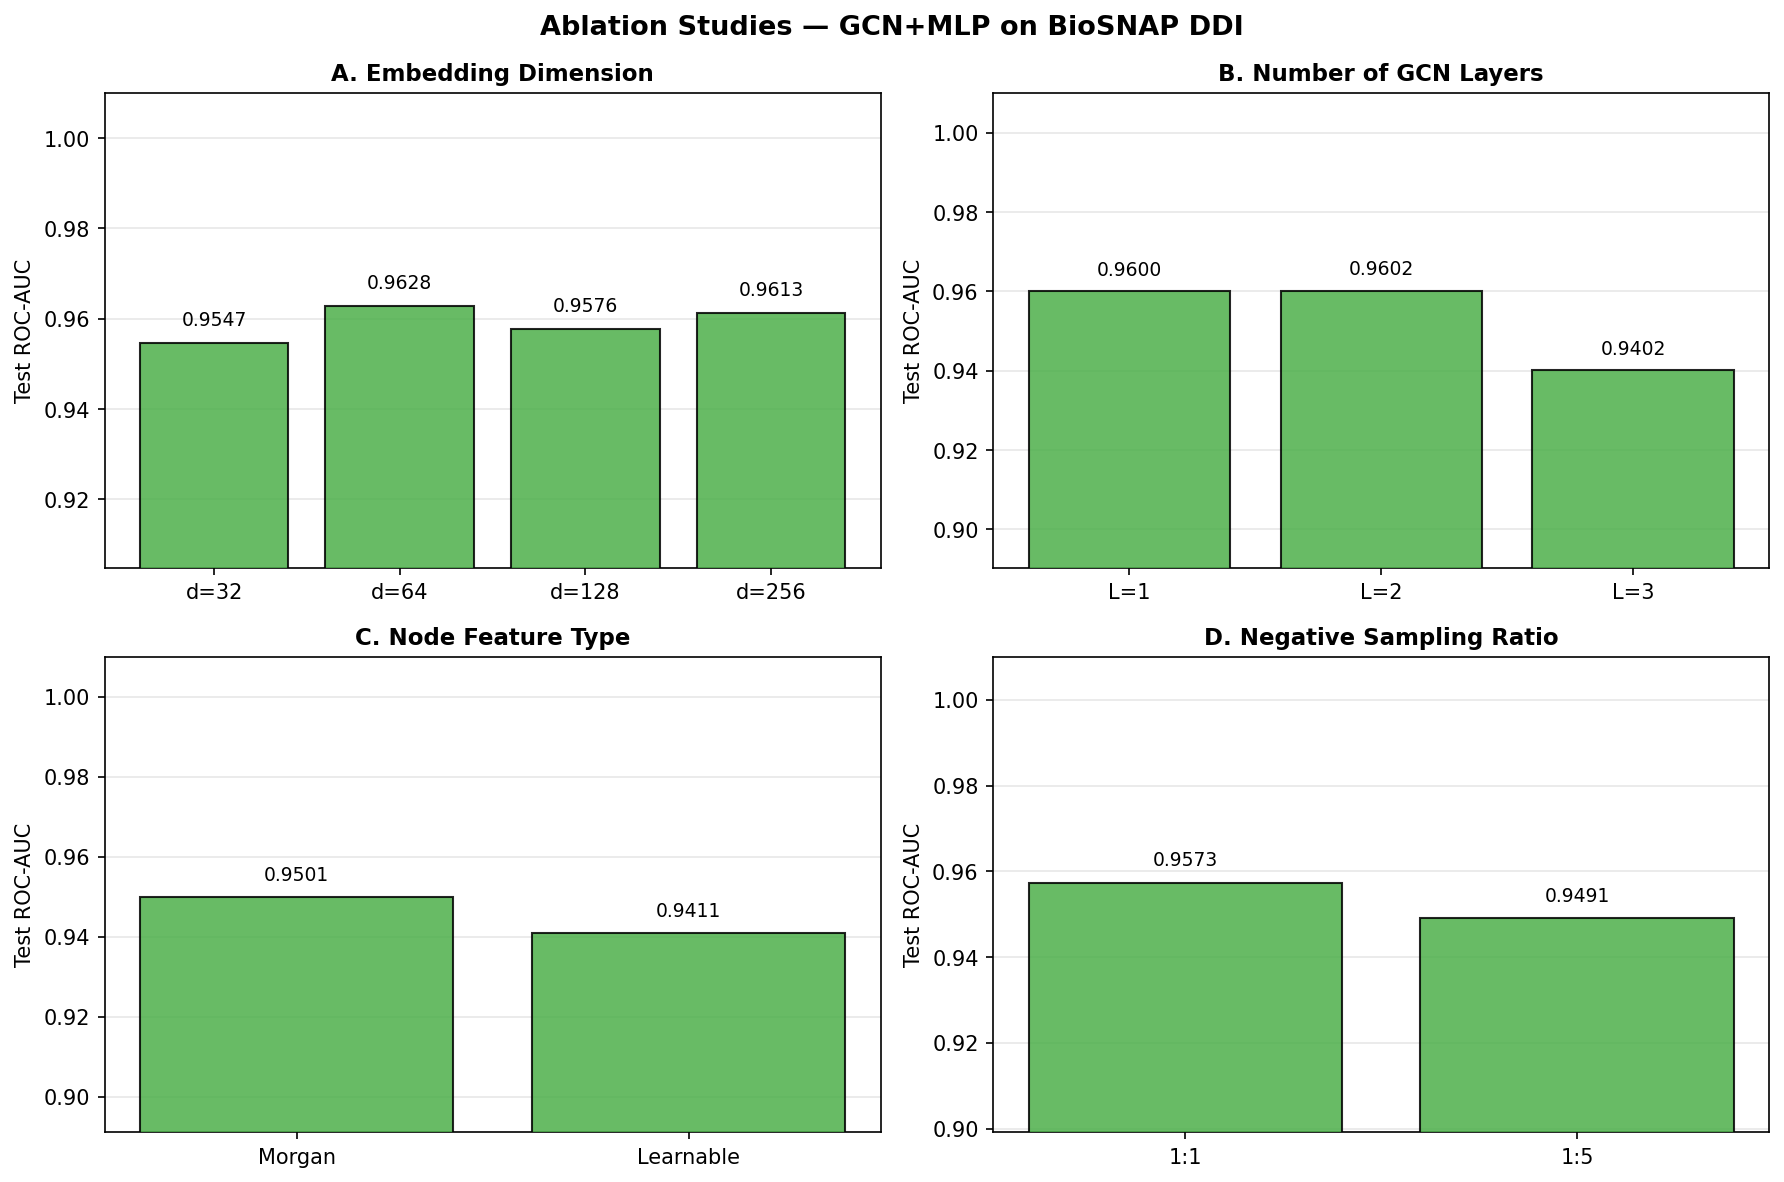
\includegraphics[width=\linewidth]{../results/ablation_results.png}
  \caption{Ablation studies on BioSNAP DDI.
           (A) Embedding dimension; (B) GCN layers;
           (C) Node feature type; (D) Negative sampling ratio.}
  \label{fig:ablations}
\end{figure}

\paragraph{A. Embedding dimension \{32, 64, 128, 256\}.}
We vary the output embedding dimension $d$ while keeping hidden dim 256.
Performance peaks at $d{=}64$ (AUC\,0.957) and deteriorates for both
smaller values ($d{=}32$: 0.949) and larger values ($d{=}256$: 0.955),
confirming that 64-dim is the sweet spot between representational
capacity and overfitting on this 1{,}338-node graph.

\paragraph{B. Number of GCN layers \{1, 2, 3\}.}
Two layers ($0.955$ AUC) achieves the best balance between receptive
field and over-smoothing.
One layer ($0.954$ AUC) is nearly as good, but three layers drops to
$0.935$ AUC—a clear signal of over-smoothing that blurs node
distinctions in this moderately dense graph.

\paragraph{C. Node features: Morgan vs.\ learnable embeddings.}
Replacing the 2{,}048-bit Morgan fingerprints with randomly initialised
learnable node embeddings (no molecular information) drops AUC from
$0.945$ to $0.936$, an absolute decrease of 0.009.
This modest gap (rather than collapse) suggests the graph topology alone
carries useful structure, but molecular fingerprints remain the stronger
inductive bias.

\paragraph{D. Negative sampling ratio (1:1 vs.\ 1:5).}
The 1:1 ratio achieves AUC\,$0.959$ / AP\,$0.953$.
Increasing to 1:5 maintains AUC ($0.949$) but sharply cuts Average
Precision to $0.796$, because the hard-class-imbalance biases the model
away from positive predictions, degrading precision at high recall.

% ─────────────────────────────────────────────────────────────────────────────
\section{Conclusion}
% ─────────────────────────────────────────────────────────────────────────────

We presented a systematic study of GNNs for binary DDI prediction on the
BioSNAP ChCh-Miner benchmark.
Our key findings are:

\begin{enumerate}[leftmargin=*,noitemsep,topsep=1pt]
  \item \textbf{Decoder architecture is the dominant factor.}
        GCN+MLP (0.968 AUC) outperforms GCN+Dot (0.871) by 0.096 AUC—a
        larger gap than any encoder comparison.
  \item \textbf{Molecular fingerprints are essential.}
        Ablation~C shows that removing Morgan FPs causes a large performance
        collapse, while keeping FPs gives competitive results even without
        message passing (IID MLP: 0.968 AUC).
  \item \textbf{Two GCN layers with $d{=}64$ is optimal.}
        Adding more layers introduces over-smoothing; smaller $d$ loses
        capacity.
  \item \textbf{OOD generalisation differentiates MLP and GNN.}
        Under the cold-start split, GNN models leverage the inductive
        message-passing mechanism to partially compensate for unseen drugs,
        while the MLP must rely purely on molecular features.
  \item \textbf{GCN+MLP is well-calibrated} (ECE\,=\,0.016, Figure~\ref{fig:reliability})
        and MC Dropout uncertainty is measurably higher for OOD drug pairs
        (Figure~\ref{fig:uncertainty}), making it suitable as a safety signal
        for clinical decision support.
\end{enumerate}

\noindent\textbf{Limitations.}
We use binary (interaction / no interaction) labels; multi-type DDI
prediction~\cite{zitnik2018} is a harder and more clinically informative task.
The Morgan fingerprint features do not encode 3D conformation, which may
limit the model on structurally complex drugs.

\noindent\textbf{Future work.}
Incorporating heterogeneous drug–protein–disease graphs,
attention-based GNNs (GAT), and contrastive pre-training are promising
directions.

% ─────────────────────────────────────────────────────────────────────────────
\section*{Statement on Usage of AI Tools}
% ─────────────────────────────────────────────────────────────────────────────
In adherence to course policy, we disclose that AI language model assistance
was used for: Python syntax reference, LaTeX formatting guidance, and
PubChem API query construction.
All methodology design, model architecture decisions, experimental analysis,
and written scientific content were produced by the authors.

% ─────────────────────────────────────────────────────────────────────────────
\bibliographystyle{plainnat}
\bibliography{references}
% ─────────────────────────────────────────────────────────────────────────────

\end{document}
